\section{The Hardware/Software Interface}

The CNN accelerator is exposed to the HPS as a 16-bit memory-mapped peripheral.
The HPS software stages model parameters and input data in a scratchpad memory,
programs the control registers, and polls the status registers until execution
completes. The MMIO wrapper then replays the staged data into the original
\texttt{system\_top} streaming datapath.

The interface uses two address regions:
\begin{itemize}
\item \textbf{Memory space} (\texttt{address[19] = 0}): 16-bit scratchpad storage
\item \textbf{Configuration space} (\texttt{address[19] = 1}): 16-bit control and status registers
\end{itemize}

\subsection{Register Map}

All registers are 16 bits wide. Table~\ref{tab:mmio-reg-map} summarizes the
register interface exposed by the MMIO wrapper.

\begin{table}[h]
\centering
\small
\begin{tabular}{|l|c|c|p{7.2cm}|}
\hline
\textbf{Register} & \textbf{Index} & \textbf{Access} & \textbf{Description} \\
\hline
\texttt{CONTROL} & 0 & WO & start model load, start inference, clear status \\
\hline
\texttt{STATUS} & 1 & RO & busy flag, model-loaded flag, done flag, predicted class \\
\hline
\texttt{CONV\_CFG\_BASE} & 2 & RW & base halfword address of convolution configuration segment \\
\hline
\texttt{CONV\_CFG\_LEN} & 3 & RW & number of 32-bit words in convolution configuration segment \\
\hline
\texttt{CONV\_WT\_BASE} & 4 & RW & base halfword address of convolution weight segment \\
\hline
\texttt{CONV\_WT\_LEN} & 5 & RW & number of 32-bit words in convolution weight segment \\
\hline
\texttt{FC\_BIAS\_BASE} & 6 & RW & base halfword address of FC bias segment \\
\hline
\texttt{FC\_BIAS\_LEN} & 7 & RW & number of 32-bit words in FC bias segment \\
\hline
\texttt{FCW\_BASE} & 8 & RW & base halfword address of FC weight segment \\
\hline
\texttt{FCW\_LEN} & 9 & RW & number of 32-bit words in FC weight segment \\
\hline
\texttt{IMAGE\_BASE} & 10 & RW & base halfword address of input image segment \\
\hline
\texttt{IMAGE\_LEN} & 11 & RW & number of 32-bit words in input image segment \\
\hline
\texttt{PREDICT} & 12 & RO & latched predicted class \\
\hline
\texttt{IF\_ERROR} & 13 & RO & interface error flags \\
\hline
\end{tabular}
\caption{MMIO register map.}
\label{tab:mmio-reg-map}
\end{table}

\subsection{Register Fields}

Table~\ref{tab:mmio-fields} lists the meaning of each implemented control and
status bit.

\begin{table}[h]
\centering
\small
\begin{tabular}{|l|l|p{8.1cm}|}
\hline
\textbf{Register} & \textbf{Bits} & \textbf{Meaning} \\
\hline
\texttt{CONTROL} & bit 0 & start model preload replay \\
\hline
\texttt{CONTROL} & bit 1 & start inference replay \\
\hline
\texttt{CONTROL} & bit 2 & clear \texttt{predict\_done} and \texttt{IF\_ERROR} \\
\hline
\texttt{CONTROL} & bits 15:3 & reserved, write zero \\
\hline
\texttt{STATUS} & bit 0 & reserved \\
\hline
\texttt{STATUS} & bit 1 & replay engine busy \\
\hline
\texttt{STATUS} & bit 2 & model preload complete \\
\hline
\texttt{STATUS} & bit 3 & inference complete \\
\hline
\texttt{STATUS} & bits 7:4 & predicted class \\
\hline
\texttt{STATUS} & bits 15:8 & reserved \\
\hline
\texttt{PREDICT} & bits 3:0 & predicted class \\
\hline
\texttt{PREDICT} & bits 15:4 & reserved \\
\hline
\texttt{IF\_ERROR} & bit 0 & model load requested while busy \\
\hline
\texttt{IF\_ERROR} & bit 1 & inference requested while busy \\
\hline
\texttt{IF\_ERROR} & bit 2 & inference requested before model load completed \\
\hline
\texttt{IF\_ERROR} & bit 3 & low halfword scratchpad read out of range \\
\hline
\texttt{IF\_ERROR} & bit 4 & high halfword scratchpad read out of range \\
\hline
\texttt{IF\_ERROR} & bits 15:5 & reserved \\
\hline
\end{tabular}
\caption{Implemented control and status bit definitions.}
\label{tab:mmio-fields}
\end{table}

\subsection{Scratchpad Address Map}

The software stores all staged data in the scratchpad memory before writing the
\texttt{CONTROL} register. The scratchpad is 16-bit addressed, so each logical
32-bit word occupies two consecutive halfword locations. The default layout is
shown in Table~\ref{tab:mmio-scratchpad}.

\begin{table}[h]
\centering
\small
\begin{tabular}{|l|c|c|l|}
\hline
\textbf{Segment} & \textbf{Base (halfwords)} & \textbf{Length (32-bit words)} & \textbf{Content} \\
\hline
\texttt{conv\_cfg} & 0 & 45 & convolution configuration \\
\hline
\texttt{conv\_wt} & 90 & 225 & convolution weights \\
\hline
\texttt{fc\_bias} & 540 & 10 & fully-connected bias \\
\hline
\texttt{fcw} & 560 & 864 & fully-connected weights \\
\hline
\texttt{image} & 2288 & 1024 & input image \\
\hline
\end{tabular}
\caption{Default scratchpad layout.}
\label{tab:mmio-scratchpad}
\end{table}

\begin{figure}[h]
\centering
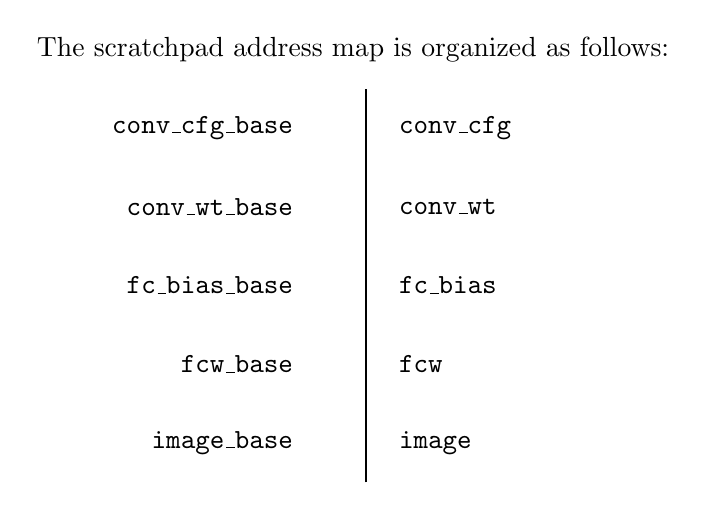
\begin{tikzpicture}[x=1cm,y=1cm]
\node[anchor=west] at (0,5.8) {The scratchpad address map is organized as follows:};

\node[anchor=east] at (3.5,4.8) {\texttt{conv\_cfg\_base}};
\node[anchor=east] at (3.5,3.8) {\texttt{conv\_wt\_base}};
\node[anchor=east] at (3.5,2.8) {\texttt{fc\_bias\_base}};
\node[anchor=east] at (3.5,1.8) {\texttt{fcw\_base}};
\node[anchor=east] at (3.5,0.8) {\texttt{image\_base}};

\draw[thick] (4.3,0.3) -- (4.3,5.3);

\node[anchor=west] at (4.6,4.8) {\texttt{conv\_cfg}};
\node[anchor=west] at (4.6,3.8) {\texttt{conv\_wt}};
\node[anchor=west] at (4.6,2.8) {\texttt{fc\_bias}};
\node[anchor=west] at (4.6,1.8) {\texttt{fcw}};
\node[anchor=west] at (4.6,0.8) {\texttt{image}};
\end{tikzpicture}
\caption{Scratchpad memory organization.}
\label{fig:mmio-address-layout}
\end{figure}

\subsection{Transaction Sequence}

Each logical 32-bit word is written into the scratchpad as two consecutive
16-bit halfwords. The MMIO wrapper reconstructs the original 32-bit word before
forwarding it to the accelerator input stream.

One inference transaction proceeds as follows:
\begin{enumerate}
\item Write preload data and input image into the scratchpad memory.
\item Program the base and length registers.
\item Write \texttt{CONTROL[0]} to start model loading.
\item Poll \texttt{STATUS[2]} until model loading completes.
\item Write \texttt{CONTROL[1]} to start inference.
\item Poll \texttt{STATUS[3]} until inference completes.
\item Read \texttt{PREDICT} and \texttt{IF\_ERROR}.
\end{enumerate}
